
%(BEGIN_QUESTION)
% Copyright 2011, Tony R. Kuphaldt, released under the Creative Commons Attribution License (v 1.0)
% This means you may do almost anything with this work of mine, so long as you give me proper credit

%An Allen-Bradley Logix5000 PLC is used to control the starting and stopping of an air compressor based on momentary-contact pushbutton switch inputs as well as high and low pressure switches (PSH and PSL, respectively).  Analyze this program and explain how it is supposed to work:

En Allen-Bradley Logix5000 PLS blir brukt til å starte og stoppe en luftkompressor. Denne styres av impulsbrytere i tilleg til høy og lavtrykks brytere (PSH og PSL). Analyser programmet for forklar hvordan det skal virke. 

$$\includegraphics[width=15.5cm]{i02346x01.eps}$$

\filbreak

$$\includegraphics[width=15.5cm]{i02346x02.eps}$$

Ha spesiell fokus på å besvare følgende spørsmål. 

\begin{itemize}
\item{$\bullet$} Avgjør den normale posisjonen til bryterene som er tilkoblet PLS-en. (Om de er NO eller NC) Ut fra funksjonen de har i programmet. 
\item{$\bullet$} Hvorfor er det viktig at en akumulerende timer blir brukt til å kalkulere total driftstid? 
\medskip

\vskip 20pt \vbox{\hrule \hbox{\strut \vrule{} {\bf Suggestions for Socratic discussion} \vrule} \hrule}


\underbar{file i02346no}
%(END_QUESTION)





%(BEGIN_ANSWER)

Input switch electrical ``normal'' statuses:

\begin{itemize}
\item{$\bullet$} {\bf Start} = NO
\item{$\bullet$} {\bf Stop} = NC
\item{$\bullet$} {\bf PSL} = NC
\item{$\bullet$} {\bf PSH} = NC
\item{$\bullet$} {\bf Reset} = NO
\end{itemize}
%(END_ANSWER)





%(BEGIN_NOTES)

The RTO timer instruction is configured to reach its end-count every hour of compressor run time.  It self-resets, with the counter instruction keeping tabs on how many timer cycles (how many hours) the compressor has run.  It is important that an RTO timer instruction is used, so that it will continue to accumulate time even if the compressor runs for less than an hour.

\vskip 10pt

The maintenance warning light turns on when the accumulated run time equals or exceeds 250 hours.

%INDEX% PLC, ladder logic program analysis and explanation

%(END_NOTES)


